\documentclass[en]{../../../eplnotes}

\hypertitle{network2-INGI2142}{8}{INGI}{2142}
{Houtain Nicolas, Gorby Nicolase Kabasele Ndondas}
{Olivier Bonaventure}
$$$$

\section{Evolution of the internet QoS and support for soft real-time
applications}

(\textit{In this paper, we review several mechanisms and frameworks
    proposed to provide network- and application-level quality of
service (QoS) in the next-generation Internet})


\subsection{Internet QoS}

Real-time applications require special support from network such
as realiability, timeliness and guaranteed delivery. The degree of
tolerance to each of these parameters varies from one application to
another.

Most of application are based on the TCP which provides reliable data
delivery service \textbf{without guaranteeing any delay and bounds}.


\begin{description}
    \item[QoS] : the capability to provide resource
        assurance and service differentiation in a network.
\end{description}

\subsubsection{Real-time application and QoS need}

$/!\backslash$ Qos cannot be solve by only adding more bandwidth
(\textit{overprovisionning}), because real-time applications requires
also garantees on delay, jitter and packet loss.

In addition, in a network there is a disparity of available bandwidths,
therefore there is a need for prioritization and protection of real-time
and mission-critical data packets at the edge routers.

$\to$ Actually approach of combining overprovisionning and
installing specific service classes. 

Advantage Qos in network :
\begin{itemize}
    \item Provide prioritization and protection to chosen traffic streams.
    \item Protect time-critival packets in case of congestion
\end{itemize}

\begin{center}
    (\textit{
    The next-generation Internet should be designed to recognize
    the service requirements of each application so that a specific
    “service class” can be assigned to each flow from these
    applications instead of putting them all in the best-effort
service.})
\end{center}



\subsubsection{Different types of QoS-dependent applications}
\begin{enumerate}
    \item \begin{itemize}
        \item Interactive : human-human or human-machine applications an
            may depend on a number of QoS parameters such as bandwidth, delay, jitter and loss.
            (IP-telephone call need an e2e delay less than 300ms)
        \item Non-interactive : Typically only need bandwidht to
            provride reasonable performance
    \end{itemize}

    \item \begin{itemize}
        \item Elastic : Do not require QoS support, only best-effort
            service and transport reliability (by using TCP)
        \item Inelastic : QoS guarantees from the underlying network for
            a certain performance level.
    \end{itemize}

    \item \begin{itemize}
        \item Tolerant : Need QoS requirement but with ranges or levels
            that can allow the application to run even if the optimal QoS
            level are not provided.
        \item Intolerant : 
    \end{itemize}

    \item \begin{itemize}
        \item Adaptive : Try to maintain the perceived quality at an
            acceptable level, even under poor network condition. (ex:
            lowering resolution of the transmission)
        \item Non-adaptive : Can tolerate some QoS degradation but this
            directly affects the quality perceived by an end user.
    \end{itemize}

    \item \begin{itemize}
        \item Realtime : Have more strict requirement on QoS and usually
            employ adaptive techniques to cope with network transients.
            (Need short delay)
        \item Streaming : Can delay their payback point with the maximun
            delay of the network.
            (Need bandwidth to be efficient and minimun bandwidth to
            work)
    \end{itemize}

    \item \begin{itemize}
        \item Multimedia : 
        \item Computation :
    \end{itemize}
\end{enumerate}

Notes to put :

Main requirement : delay, bandwidth and packet losses.

Check source/destination with MAC adresses and application
classification by port (80/443 for HTTP and HTTPS)

\subsection{QoS requirements}

\subsubsection{QoS parameters}

\begin{itemize}
    \item Throughput : effective number of data units trans-
        ported per unit time (e.g., bits/second).
        $\to$ A rate ($r$) and burst size ($b$). (See token bucket)
    \item Delay : between departure to the arrival.
        $\to$ A maximum delay bound ($D_{max}$)
    \item Jitter : delay variation.
        $\to$ A maximun variation boud ($J_{max}$).
    \item Loss : probability of loss
    \item Reliability 
\end{itemize}

\subsubsection{Service commitment}

\subsubsection{Admission control}


\subsection{Building block for providing network-level QoS}

\subsubsection{Scheduling}
\begin{itemize}
    \item FIFO : no suitable for providing service differentiation and
        QoS guarantees (because no differentiation)
    \item Priority scheduling : Can can starvation to lower-priority
        classes
    \item Generalized processor sharing (GPS) : Priority scheduling but
        solve the starvation issues but GPS cannot be implement in
        practice.
    \item Weighted fair queueing (WTQ) : Approximate GPS by calculate
        the finish time for each packet by using weight by flow ($\phi$).
        $$ F_i^k = max[f_i^{k-1}, R(t)] + \frac{L_i^k}{\phi_i} $$

        $\to$ Use in most router because WTQ allows a faire share of
        bandwith among all the queueys. But WTQ need to maintain
        per-flow queueing information since an appropriate weight for
        each flow must be generated.

    \item Class-based queueing (CBQ) : create a sharing tree fo all
        classes to be supported for a link.

        In practice, it is use with priority scheduling
\end{itemize}

\subsubsection{Buffer management}
Random early detection (RED) gateways are often employed to avoid
congestion in packet networks.

Weighted RED (WRED) is a variant of RED where packets
with higher IP precedence bits have a lower probability of
being dropped than packets with lower precedence.
$\to$ WRED can make differentiated drop probabilities.

\paragraph{Note:} IP precedence = 

\subsubsection{Policing}

The token buckets are the most common mechanisms used for policing
traffic at a network node. 

A token bucket has a bucket of depth $b$ and generates tokens at the
rate of $r$ . Each arriving packet consumes a token (or a number of tokens
directly proportional to the packet size, depending on implementation)
before it can be transmitted into the network.

\textbf{in-profile} if bit rate $\leq r$ and burst size $\leq b$,
\textbf{out-of-profile} else.

\begin{figure}[h]
    \centering
    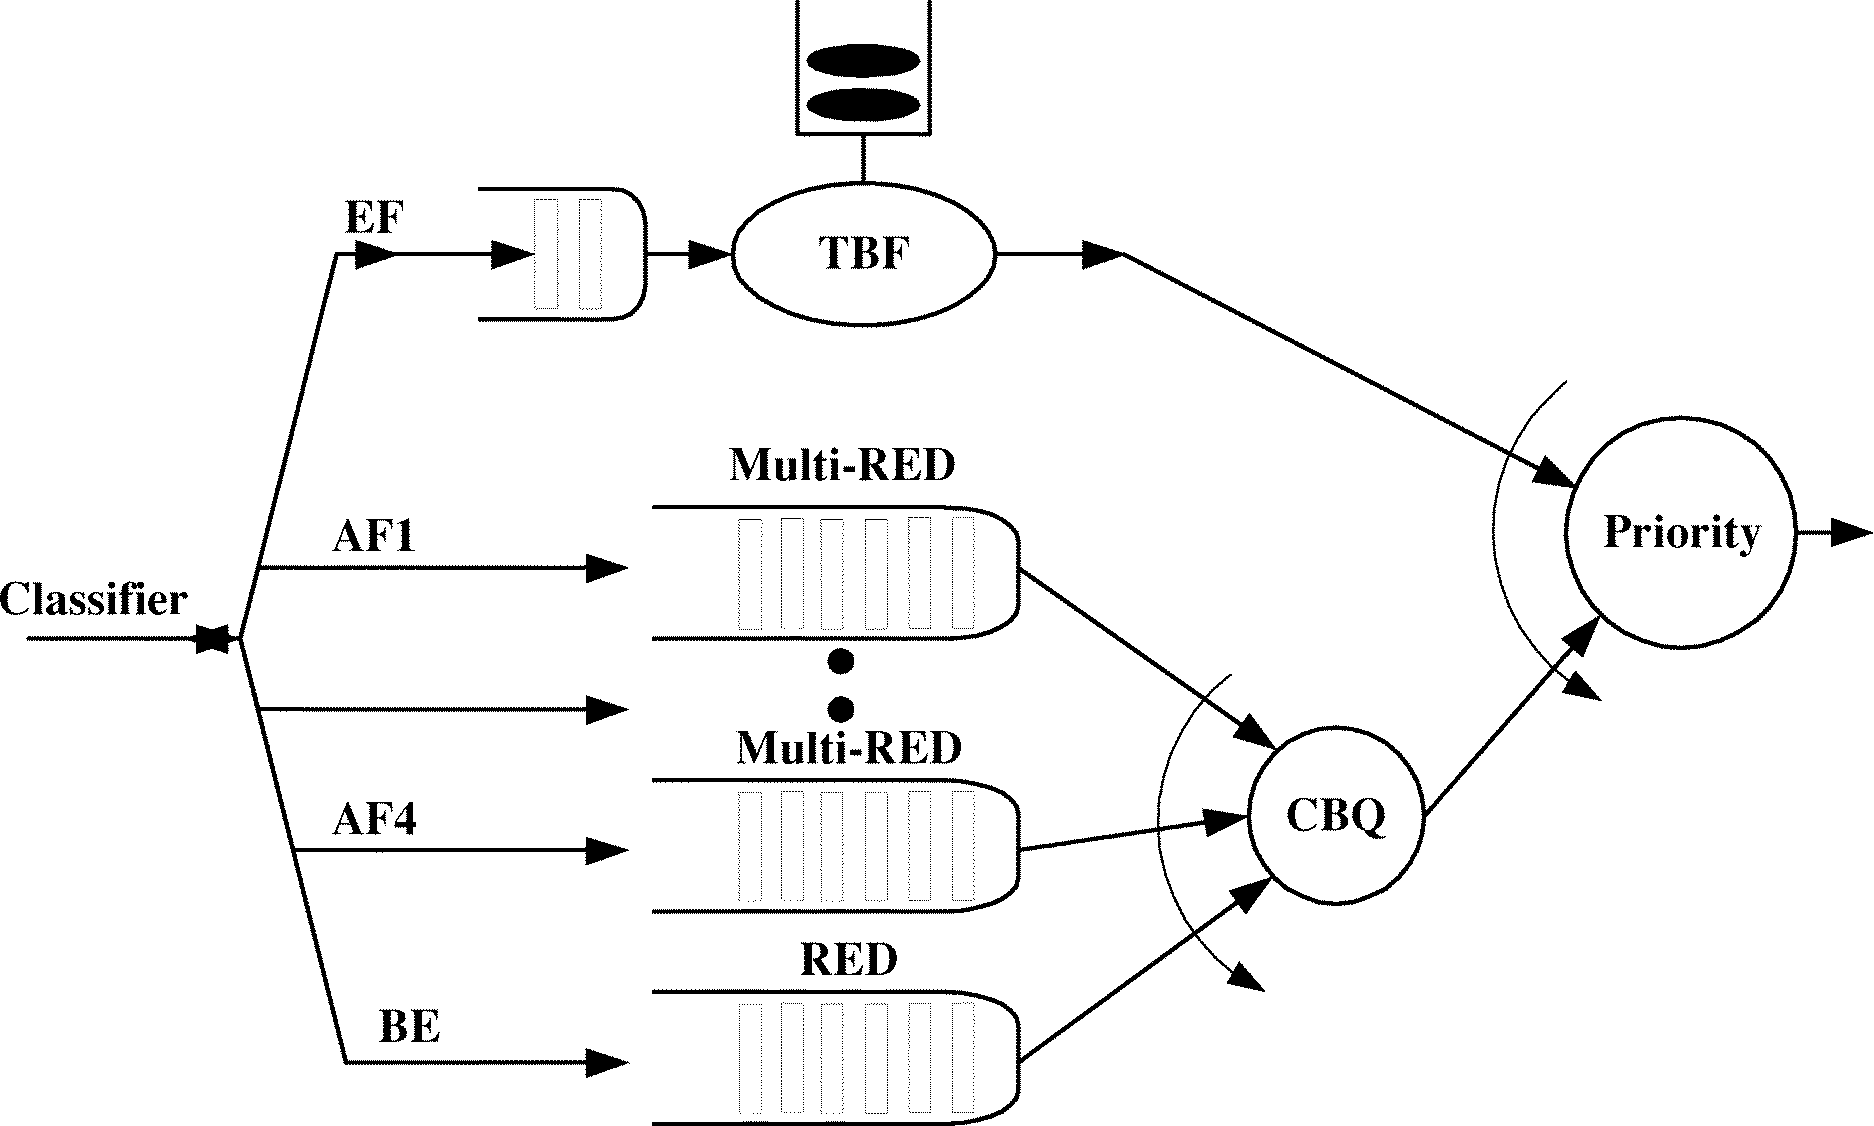
\includegraphics[width=8cm]{img/QoS_building-blocks.png}
    \caption{Implementation of QoS building blocks}
\end{figure}

\subsection{ATM}


\subsection{IP precedence and ToS}


\subsection{IntServ and RSVP}

\subsubsection{IntServ Model}
IntServ was designed to provide QoS to individual flows
(or an individual session in case of multicast applications).

IntServ provisions virtual paths for each flow and sets up
the required resources on these virtual paths. 

However,
routing is not affected by these virtual paths, and they follow
the default routing paths provided by the Internet routing
protocols.

$\to$ It's done by using RSVP.


\paragraph{Warning} Routing is not affected by these virtual path
because the reservation follows the entire route of the data packet.
\textbf{If route change, reservation is redone} (because of soft-state).


\subsubsection{Services classes}

IntServ services classes :
\begin{itemize}
    \item[-] Basic best-effort
    \item[+] Guaranteed Service (GS) : Used by applications that 
    requires strict bounds on the e2e delay. It use a token bucket
    proffile$(r,b)$ where
    \begin{itemize}
    	\item Minimun sending rate ($r$) 
    	\item Minimun burst size of the traffic ($b$)
    \end{itemize}
    Routers allocate a forwarding rate of R for each session with
    a request if rate < R.
    \item[+] Controlled load (CL) : Experience small queueing delays,
    low loss and overall performance as if the network is not loaded.

\end{itemize}


\subsubsection{Reservation with RSVP}
\begin{enumerate}
    \item Sender sending \textbf{PATH message} (each 30sec) that carries :
        \begin{itemize}
            \item Tspec : Traffic specification object that describes
                the traffic profile. 

                rate ($r$), bucket ($b$), peak rate ($p$), minimum unit
                ($m$) and max packet size ($M$).

            \item ADspec : Advertisement specification object wich
                compute the accumulated QoS parameters along the e2e
                path.

            \item Phop : It's the path to join the receiver. The
                receiver juste send by the reverse path.

                \begin{itemize}
                    \item[Note:] There is a flowtable on each router to
                        know the ``reverse'' path
                \end{itemize}
            
        \end{itemize}

    \item Receiver replies back with \textbf{RESV message} that carries :
        \begin{itemize}
            \item Rspec : Reservation specification
        \end{itemize}

    \item[Accepted] : if accepted by all routers along the path.

        $\to$ Setut actual reservation and filters ont these router

    \item[Error] : corresponding router send PATHerr or RESVerr

    \item[End] : PATHtear and RESVtear message are sent to remove
        reservation states
\end{enumerate}


\paragraph{Filter}
\begin{itemize}
    \item Fixed filter :
    \item Shared filter :
    \item Wildcard filter :
\end{itemize}

\subsubsection{Evalutation of the IntServ model}


\subsection{Differentiated services}

\subsubsection{Background}







\end{document}
